\chapter{Gestion des fichiers}

\begin{multicols}{2}  

\section{Les fichiers}

Qu'est-ce qu'un fichier ?

\begin{itemize}
\item 
Un fichier est une suite de données structurées codées sur un support.
\item 
Les fichiers sont la plupart du temps conservés sur des \emph{mémoires de
masse} tels que les  disques durs. 
\item 
Les fichiers sont classés dans des  \emph{répertoires}, chaque
répertoire peut contenir d'autres répertoires, formant ainsi une
\emph{organisation arborescente} appelée \emph{système de fichiers}.
\end{itemize}

\FIGURE{tree-korn0102.png}{un système de fichiers}


Autrefois les systèmes d'exploitation prenaient en charge différents
types de fichiers :
\begin{itemize}
\item les fichiers de texte, composés de lignes de taille variable ;
\item les fichiers séquentiels, composés d'enregistrements
\item les fichiers relatifs, contenant des enregistrements accessible directement par leur numéros (le système d'exploitation fournit des fonctions d'accès du type : ``lire l'enregistrement numéro 25'')
\item les fichiers indexés, dont les enregistrements comportent une
  \emph{clé} (par exemple la plaque d'immatriculation pour un fichier de cartes grises). On peut alors demander à lire l'enregistrement concernant la plaque
  ``1234AB56''.
\item ...
\end{itemize}

De nos jours, la plupart des systèmes connaissent un seul type : les
fichiers sont une séquence d'octets, avec des opérations
(\texttt{read, write}) pour lire et écrire à partir d'une position
courante, et se positionner (\texttt{seek}) à un endroit déterminé
(numéro d'octet).  Les fonctionnalités des fichiers indexés, par
exemple, sont fournies par des bibliothèques spécialisées (voir par exemple la page de manuel  \texttt{dbopen}).






\section{Les disques}

Les disques magnétiques que nous connaissons dérivent des mémoires à
tambours magnétiques, des cylindres en rotation couverts d'un enduit
ferro-magnétiques, avec des têtes magnétiques qui
assuraient la lecture et l'écriture.

\FIGURE{magnetic-drum.jpeg}{ancêtre : le tambour magnétique}

En 1953, un ingénieur d'IBM a eu l'idée de superposer des plateaux sur
un axe, et d'ajouter une tête de lecture-écriture mobile, portée par
un bras. Le bras pouvait changer de disque en moins d'une seconde.

\FIGURE{RAMAC-EngProtoType.jpeg}{Prototype d'IBM}

La production commerciale du RAMAC 305 (Random Access Method of
Accounting and Control) a commencé en juin 1957.


Caractéristiques: 
\begin{itemize}
\item 59 disques de 24 pouces
\item 2 têtes pouvant se déplacer d'un plateau à l'autre
\item capacité totale de 5 megaoctets.
\item prix de 10000 dollars par megaoctet.
\end{itemize}

% \FIGURE{5MB-Hard-Disk-in-1956.png}{Livraison du premier RAMAC 305, en 1956)}

De nombreuses améliorations ont été apportées : 
\begin{itemize}
\item l'utilisation de
plusieurs têtes de lectures portées par un même bras (une par face de
disque) dispense de déplacer la tête d'un disque à l'autre. 
\item un coussin d'air permet de ``faire flotter'' les têtes en
  évitant qu'elles rentrent en contact avec le disque, incident appelé
  ``atterrissage'' qui endommage irrémédiablement la surface magnétique.
\end{itemize}
L'augmentation de la précision mécanique du mouvement des têtes et de
la vitesse de rotation du disque (entre 3600 et 15000 tours/mn) a
permis d'augmenter la capacité : 5 Mo en 1956, 1 Go en 1982, 25 Go en
1998, 500 Go en 2005, 2 To en 2009, 4 To en 2011.




\FIGURE{DiamondMax-80GB-Internal-Hard-disk.png}{Une unité de disque 
récente (80GB), début du siècle}

De nos jours, on trouve des disques de capacité 4 To en format 3 pouces et demi
(Hitachi 7K4000).



\subsection{Disque, tête}

\FIGURE{tete-lecture.png}{Disque, tête de lecture, bras}

La position d'une tête  définit  une \emph{piste}

\FIGURE{piste.png}{Une piste}

Les pistes sont découpées  en \emph{secteurs} (angulaires)

\FIGURE{secteur.png}{Un secteur}

Un secteur contient (pour simplifier) un  \emph{bloc de données}.

\FIGURE{bloc.png}{Un bloc}


Changer de piste implique un  \emph{mouvement} de la tête, changer de secteur
une rotation.


\subsection{Avec plusieurs plateaux}

\FIGURE{harddisk.png}{Un axe, un bras, plusieurs plateaux}

On appelle \emph{cylindre} l'ensemble des pistes pour une position
définie du bras.

\FIGURE{dd1.png}{\emph{Cylindre} = pistes \\ pour une position du bras}

\begin{itemize}
\item Accéder à un autre cylindre implique un mouvement du bras, qui est lent (à l'échelle de l'ordinateur)
\item Changer de tête se fait par commutation électronique d'une tête à l'autre.
\end{itemize}



À retenir : le disque magnétique est un médium à \emph{temps d'accès
  non uniforme} : le délai pour accéder à une information dépend de la
position de cette information, et de la position courant des têtes de
lecture.

Dans ce délai il faut intégrer
\begin{itemize}
\item le déplacement du bras (sélection du cylindre)
\item la rotation (sélection du bloc)
\end{itemize}
Le temps de commutation (sélection de la piste) est négligeable.

Le délai le plus long vient du mouvement de la tête.  Il en résulte un principe de localité : pour minimiser les déplacements de tête, et donc les temps d'accès, il vaut mieux grouper les données sur des cylindres proches.

\subsection{Quelques chiffres}


\begin{tabular}{rl}
couche magnétique & 10-20 nm \\
vitesse de rotation & 5400-15000 tours/min \\
capacité & 120 GB -2 TB \\
temps d'accès & 2-15 ms \\
vitesse de transfert & 70 MB/sec (7200 t/min) 
\end{tabular}


\section{Gestion des entrées/sorties sur disque}


\subsection{Sur un système mono-tâche}

Sur un système mono-tâche : il n'y a pas (trop) de problème,
on déplace la tête à la demande là où on en a besoin.

Bien évidemment les performances sont meilleures 
 si les blocs d'un fichier  sont regroupés.  Il est donc 
prudent, parfois, de \emph{défragmenter} les systèmes
de fichier pour regrouper les blocs.

Autrefois on profitait de la sauvegarde pour copier
le disque original, fichier par fichier, sur un disque vierge, 
ce qui regroupait les blocs. Le disque original était alors démonté
et conservé comme sauvegarde.

Bien entendu, une telle sauvegarde se faisait dans le cadre d'une
maintenance planifiée : pendant quelques heures l'ordinateur était
inaccessible aux utilisateurs.


\subsection{Sur un système multitâche}

Sur un système multitâches il est possible que plusieurs processus
soient bloqués pour avoir demandé une opération sur le même disque.
Il y a donc plusieurs demandes en attente : laquelle servir en premier ?
C'est le problème d'\emph{ordonnancement des mouvements du bras du disque}.

\subsection{E/S : Premier arrivé, premier servi}



Une première politique  peut être facilement imaginée : exécuter les demandes
dans l'ordre où elles ont été effectuées. 


Exemple : 
trois processus qui lisent et traitent des données situées dans des blocs
consécutifs : P1 commence au bloc 100, puis 101, 102, etc.  Idem pour P2 et P3 qui commencent respectivement à 200 et 500.



Déroulement :
\begin{itemize}
\item P1 demande la lecture du bloc 100, qui commence à s'exécuter; P2 demande le bloc 200, P3 le bloc 400
\item la lecture se termine, la lecture du bloc 200 s'exécute,  P1 demande le bloc 101. 
\item la lecture se termine,  la lecture du bloc 500 s'exécute, P2 demande le bloc 201.
\item  le lecture du bloc  101 commence, P3 demande le bloc 501, ...
\item etc.
\end{itemize}
Successivement, on lit donc les blocs 100, 200, 500, 101, 201, 501, 102, ...

Cette politique ``premier arrivé - premier servi'' est
\begin{itemize}
  \item \emph{simple} à mettre en oeuvre
 \item \emph{équitable} ...
 \item mais \emph{pas efficace}
\end{itemize}



\subsection{E/S : plus court déplacement}

Cette politique consiste à exécuter la requête qui demandera le moindre déplacement.

Sur le même exemple, après avoir lu les blocs 100 et 200 on a en attente des demandes pour 101 et 500. La position 101 est la plus proche de la position courante (200), on retourne donc à P1.

Il en résulte l'ordre suivant : 100, 200, 101, 201, 102, 202 ...
et on constate que les lectures de P3 ne sont pas faites en raison de la coalition entre P1 et P2.

En résumé, la politique ``déplacement le plus court'' est
\begin{itemize}
  \item \emph{simple} à mettre en oeuvre
 \item \emph{efficace} ...
 \item mais \emph{pas équitable}
\end{itemize}


\subsection{Politique de l'ascenseur}

La politique dite ``de l'ascenseur'' est un compromis intéressant.

L'algorithme de gestion est à deux phases
\begin{itemize}
\item dans la phase montante, on traite la requête qui concerne le plus petit
de bloc strictement supérieur à la position courante. SI il n'y en a pas, on passe en phase descendante.
\item dans la phase descendante,  on traite la requête pour le plus grand numéro de bloc strictement inférieur à la position courante. Si il n'y en a pas on passe en phase montante.
\end{itemize}

Déroulement :
\begin{itemize}
\item  ($\Uparrow$)   100,   200,   500, 
\item   ($\Downarrow$)   201,   101, 
\item   ($\Uparrow$) 202, 501,
\item    ($\Downarrow$) 203, 102,
\item   ($\Uparrow$) 204, 502  
\item ($\Downarrow$) ...
\end{itemize}


La politique de l'``ascenseur'' est 
\begin{itemize}
 \item \emph{assez équitable} ...
 \item \emph{assez efficace}
\end{itemize}


\subsection{E/S : Deadline driven disk scheduler}


Une idée plus moderne :  on fixe un délai maximum, après lequel
l'exécution d'une requête devient urgente.

Algorithme :
\begin{itemize}
\item si il y existe des requêtes urgentes, on traite la plus ancienne
(qui est aussi la plus urgente)
\item si il n'y en a pas, on traite la requête qui demande le moins de
  mouvement.
\end{itemize}

La politique ``deadline driven scheduling'' est
\begin{itemize}
 \item \emph{efficace}
 \item et \emph{équitable}
  \item ... et brevetée
\end{itemize}

\begin{exercice}
Traduire en français correct le titre du brevet \emph{United States Patent 5787482} de 1998 :

\texttt{
Subject: Deadline driven disk scheduler method and
  apparatus with thresholded most urgent request queue scan window}
\end{exercice}


\subsection{Conclusion}
\begin{itemize}
\item Une problématique spécifique, par rapport à la gestion des données en mémoire, est de tenir compte du temps d'accès aux données, qui n'est pas
uniforme.
\item   Il y a un compromis à trouver entre 
\emph{efficacité}
et \emph{équité}
\item  quelques heuristiques simples pour l'ordonnancement :
\begin{enumerate}
\item premier arrivé, premier servi
\item plus court déplacement
\item ascenseur
\item \emph{deadline scheduling}
\end{enumerate}
\end{itemize}



\section{Systèmes RAID}

\subsection{Principe et objectifs}

Les systèmes RAID (\emph{Redundant array of inexpensive disks}) sont composés
de plusieurs disques groupés dans un boîtier ou un
\emph{rack}\footnote{Boîtier que l'on boulonne dans une armoire
  informatique de taille normalisée}.

\FIGURE{boitier-raid.jpeg}{un boitier RAID}
\FIGURE{boitier-raid-2.jpeg}{un rack RAID}


 L'objectif initial était de réaliser des systèmes
de stockage de grande capacité en combinant des ``petits'' disques bon marchés,
plutôt qu'en achetant de gros disques, qui n'étaient disponible que sur
marché du matériel professionnel, et donc beaucoup plus coûteux.


On verra que grouper des disques permet non seulement d'étendre la
\emph{capacité}, mais aussi d'améliorer la \emph{fiabilité} (par
l'introduction d'une redondance) et les \emph{performances}, en faisant
travailler les disques en parallèle.

Actuellement on traduit RAID par
Redundant Array of \emph{Independent} Disks, les systèmes n'étant pas
forcément composés de disques bon marché.


\paragraph{Connexion des disques}
\begin{itemize}
\item les disques peuvent être connectés de la manière habituelle, et
  le RAID géré par des modules spécifiques du système d'exploitation
\item les disques  peuvent être raccordés à une carte d'extension qui prend
en charge les fonctions du RAID
\item la carte mère peut intégrer la fonction RAID,
\item les disques peuvent également être intégrés à un boîtier (ou
  rack) extérieur, qui se comporte comme un disque unique.
\end{itemize}


Il existe un grand nombre de manières de combiner plusieurs disques
physiques pour réaliser un système de stockage.

\subsection{NRAID (JBOD)}

Le degré zéro du RAID consiste à ``concaténer'' de petits disques pour
un faire un gros. Par exemple, avec 4 disques de 500 Go on obtient un
système de 2 To. Les premiers secteurs du système sont sur le disque 1, les
suivants sur le disque 2, etc.

Ceci permet de répartir les données, mais n'assure aucune redondance,
d'où les noms usuels NRAID et JBOD
\begin{itemize}
\item NRAID \emph{is Not RAID}
\item JBOD  \emph{just a bunch of disks}
\end{itemize}

\begin{exercice}
Les disques sont-ils nécessairement de même taille ?
\end{exercice}

On notera qu'il est possible de mener plusieurs requêtes
d'entrées-sorties simultanément sur le système, si par chance elles
concernent des disques différents. Ceci a un impact positif sur les
performances.\footnote{par rapport à l'utilisation d'un disque unique
  de 2 To}.


En cas de défaillance d'un disque, les données sont compromises. Les
fichiers qui ont des blocs sur le disque défaillant sont
irrécupérables.




\subsection{RAID 0 : agrégation par bandes}

Le RAID 0, ou stripping, combine des disques de même taille.  A la
différence du NRAID, les données sont réparties par \emph{bandes} : le
premier bloc du système est sur le premier disque, le second sur le
second disque etc.
 
\FIGURE{raid0.png}{RAID 0 : agrégation par bandes}

Ceci permet une meilleure répartition de la charge de travail, en
tenant compte également du principe de localité : après avoir lu un
bloc on a très probablement besoin du suivant ; il est donc possible,
en parallèle, de le lire de façon anticipée. 


\FIGURE{raid0.png}{Demande de lecture 7 : \\
possibilité de \emph{lecture anticipée} de 8 et 9 \\ dans le même temps}


On ne peut pas anticiper les écritures, mais  plusieurs écritures en même temps, à condition
qu'elles se déroulent sur des disques différents.

\FIGURE{raid0.png}{\textbf{exemple} \\
lecture/écriture de 2, 6 et 11}


En cas de défaillance d'un disque les données sont irrécupérables.



\subsection{RAID 1 : miroir}

Dans une configuration en miroir, les données sont stockées en double
(ou plus).  

\FIGURE{raid1.png}{RAID 1 : miroir}


Avec 2 disques de 500 Go chacun, on fait donc un système RAID 1 de 500 Go.

L'objectif est bien sûr d'améliorer la redondance : si un
des disques tombe en panne, on peut retrouver les données sur l'autre disque.



\begin{exercice}
Si les disques ont une probabilité de panne de 5/100 par an, quelle est la
probabilité de perdre les données dans un système RAID de 2 disques ?
\end{exercice}

\begin{exercice}
Peut on faire du RAID 1 avec 3 disques ?
\end{exercice}



Toute opération d'écriture sur le système se traduit obligatoirement 
par des écritures tous les disques, menées simultanément, ce qui 
ne prend pas plus de temps qu'une seule écriture.

\FIGURE{raid1.png}{\emph{Écriture} : doit se faire en parallèle}

Par contre, puisque les données sont en double, on peut lire des blocs
à 2 adresses différentes en mêmes temps.

\FIGURE{raid1.png}{\emph{Lecture} : deux à la fois}

 Globalement, on peut donc
mener deux fois plus de lectures qu'avec un seul disque : il y a donc
un gain de performances en lecture.

\subsection{Disques de rechange, reconstruction}

Un boîtier RAID possède en général des emplacements supplémentaires 
pour des disques de rechange (\emph{spare disks}).

Par exemple un boîtier en RAID 1 à deux disques peut avoir 3
emplacements.  Normalement 2 disques (D1, D2) sont actifs et
fonctionnent en miroir, le dernier D3 est arrêté.

Si un problème est détecté sur un disque actif - par exemple D2 - le
système de disques peut encore fonctionner en mode dégradé (le
fonction miroir n'est plus assurée) sur D1. Le boîtier procède alors 
à la \emph{reconstruction} automatique du miroir : il met alors
automatiquement en route le disque D3, et y fait une copie du disque
D1 qui est encore valide. Quand cette copie est terminée, le système
fonctionne à nouveau en miroir sur D1 et D3.

En général le boîtier possède aussi une interface réseau, et fait
remonter une alerte à l'administrateur pour qu'il remplace rapidement
 le disque défectueux par un nouveau disque de rechange.


\subsection{RAID 4 : agrégation par bandes avec parité}

Le principe du RAID 4 est une amélioration du principe du miroir.
Au lieu de dupliquer les données, on utilise un système de ``parité''
qui permettra de reconstituer le disque manquant.

Partons d'un système RAID 0 à trois disques A, B, C: les trois premiers blocs
du système sont sur les premiers blocs des disques, les trois blocs
suivants sur les seconds blocs etc.  Ajoutons un quatrième disque D, sur
lequel nous stockerons, dans le Nième bloc, un ou-exclusif des Nièmes
blocs des 3 disques de données.
$$ D_n = A_n \oplus B_n \oplus  C_n $$

\FIGURE{raid4.png}{RAID  4 : agrégation par   \emph{bandes}
 avec\emph{parité}}

Si le disque A tombe en panne, il sera possible de reconstituer
son contenu. En effet, les propriétés de l'algèbre de Boole font que 
le bloc $A_n$ est le ou-exclusif des autres blocs de la 
même ``bande'' :
$$ A_n = B_n \oplus  C_n \oplus D_n $$

Le RAID 4 permet donc d'avoir de la redondance sans doubler la taille
totale des disques.  Les systèmes usuels ont 4 ou 5 disques, la place
disque nécessaire à la redondance est donc de l'ordre de 20 ou 25\%.

Il est possible de mener de front plusieurs lectures, d'où une possibilité
de gain de performances.

\FIGURE{raid4.png}{Lectures en parallèle}

Par contre, pour modifier un bloc, il faut modifier aussi le bloc ``de parité'',
et pour le calculer, il faut avoir lu les blocs de la bande. Une écriture
peut donc prendre le temps de deux accès disque.

Remarquez aussi que le disque de parité est sollicité à chaque écriture.
Il constitue donc un goulet d'étranglement.

\FIGURE{raid4.png}{
  \emph{goulet d'étranglement en écriture}\\
  (accès au disque de parité)}

\subsection{RAID 5 : agrégation par bandes avec parité répartie}

Le RAID 5 est une amélioration du RAID 4 pour mieux répartir la charge :
selon les bandes, le bloc de parité n'est pas situé sur le même disque.

\FIGURE{raid5.png}{RAID 5 : agrégation par bandes avec \emph{parité répartie }}

\FIGURE{raid5.png}{la charge en écriture est répartie}

Ceci conduit à de meilleurs performances.

\subsection{Combinaisons : RAID 10}

Les techniques vues précédemment sont combinées entre elles pour combiner, selon les besoins, redondance et performances.

Par exemple, le RAID 10 (ou RAID 1+0) est une ``grappe'' RAID 0 (stripping)
de paires de disques en miroir :


% \FIGURE{200px-RAID_10.png}{grappe RAID 1 de paires de disques en miroir}
\FIGURE{raid10.png}{RAID 1 sur disques en miroir}

%\end{multicols}

\subsection{RAID 51}

De la même façon, le RAID 51 est un miroir de deux grappes RAID 5 :

% \FIGURE{200px-RAID_51.png}{miroir entre 2 grappes RAID 5}
\FIGURE{raid51.png}{\emph{miroir} entre 2 \emph{grappes RAID 5}}

% \begin{multicols}{2}

\subsection{RAID 50}

Laissé en exercice :

\begin{exercice}
Dessinez un système de stockage RAID 50.
Comparez 
 performance et fiabilité avec le RAID 51
\end{exercice}

\subsection{Choix d'un système RAID}

Les systèmes RAID servent à réaliser des systèmes de stockages de
données, avec des objectifs de capacité, de fiabilité et de
performances qui sont supérieurs à ceux des disques individuels.
C'est une technologie qui est de nos jours indispensable en environnement
professionnel.

Les objectifs sont atteints en combinant diverses techniques : la
duplication, la répartition, la parité.

De multiples combinaisons sont possibles : pour faire le bon choix 
dans un contexte donné, il faut les comprendre.



\section{Systèmes de fichiers}

Les \emph{systèmes de fichiers} sont des structures de données,
stockées sur disque, qui représentent des fichiers, des répertoires
etc.

Vu par l'utilisateur du système (c'est à dire le programmeur d'applications),
un fichier possède un contenu, et des méta-données :

\begin{itemize}
\item sa taille
\item son propriétaire
\item les droits d'accès
\item la date de création
\item date de dernier accès
\item ...
\end{itemize}


\subsection{Fonctions du SGF}

Le Système de Gestion de Fichiers (SGF) contient des fonctions pour

\begin{itemize}
\item Manipulation des fichiers : créer/détruire des fichiers, ...
\item  Allouer de la place sur mémoires secondaires
\item Localiser des fichiers : accès au contenu
\item Sécurité et contrôle des fichiers
\item Fiabilité en cas de panne
\item ...
\end{itemize}

On s'intéresse ici à la représentation des fichiers et des répertoires sur les
disques.

\subsection{Catalogue de fichiers}

Les premiers disques avaient une capacité très faible (quelques méga octets).
Selon un principe constant en histoire de l'informatique,
\begin{quotation}
\emph{faire du vieux avec du neuf}
\end{quotation}
 ils ont été
d'abord gérés en utilisant les méthodes issues des technologies précédentes,
à savoir les bandes magnétiques.

Les bandes magnétiques sont un support à accès essentiellement
séquentiel (il existe quand même un moyen de ``bobiner'' plus vite, en
avant ou en arrière) sur lequel les fichiers sont stockés les uns
après les autres. En début de bande, on met un premier petit fichier, qui 
contient le nom de la bande, et la liste des fichiers présents.

Les premiers disques étaient gérés de la même façon (VTOC = Volume
Table of Contents, d'IBM) : au début du disque se trouve une table,
qui contient les noms, positions de départ (numéro de bloc) et taille
de chaque fichier.  On trouve aussi la liste des espaces inutilisés,
pour pouvoir allouer de nouveaux fichiers.


Cette manière de faire possède tous les inconvénients que l'on connaît
pour la gestion de la mémoire par blocs contigus : il se produit fatalement
une certaine fragmentation, et il est difficile d'allonger un fichier existant.

Par contre, pour une utilisation en mono-tâche les performances
sont très bonnes : les données d'un même fichier sont proches les unes des
autres, ce qui minimise le temps d'accès?

A noter : avec des disques de taille aussi réduite, il n'apparaît pas nécessaire
d'avoir une organisation hiérarchisées sous forme de répertoires.


\subsection{FAT : file allocation table}

Une autre solution est d'utiliser deux tables
\begin{itemize}
\item une table d'allocation qui indique les méta-données de chaque fichier, 
et la position (index) de son premier bloc ;
\item une table d'index donnant, pour chaque bloc, la position de son 
successeur.
\end{itemize}

La table d'index est chargée en mémoire au montage du disque.


Ceci permet de gérer les fichiers de manière similaire à la mémoire
paginée : les blocs d'un fichier ne sont pas contigus, ce qui fait
qu'on ne rencontre pas le problème de ``gruyérisation''.

Par contre, la dispersion sur le disque des blocs d'un même fichier
peut avoir un impact important sur les performances, parce que le
disque est un support à temps d'accès non-uniforme.

Il y a donc diverses stratégies au niveau du système pour mimimiser la
dispersion. Par exemple le disque sera géré par zones, le système
prenant soin d'essayer garder un certain pourcentage de place libre
dans chaque zone, pour pouvoir y loger de préférence les blocs
supplémentaires des fichiers qui font déjà partie de la zone.

\begin{exercice}
Soit un disque de 10 Mo, géré par blocs de 2 Ko. Quelle serait la
taille de la table d'index ?
\end{exercice}




\subsection{Tables des blocs Unix}

Unix est une vaste famille de système d'exploitations, qui supporte
une multitude de types de systèmes de fichiers.

\begin{exercice}
Sur les machines Linux regardez dans \url{/lib/modules/*/kernel/fs} la liste
des pilotes qui prennent en charge les systèmes de fichiers. Recherchez à quoi
correspondent \texttt{aufs}, \texttt{jfs}, \texttt{ntfs} ?
\end{exercice}

Dans ce qui suit
nous décrivons les principes utilisés dans les premiers systèmes Unix : 
l'espace disque comporte deux zones 
\begin{itemize}
\item les méta-données
\item les blocs de données (contenu des fichiers)
\end{itemize}


À chaque fichier est associé un \emph{i-node} (noeud d'information)
\begin{itemize}
\item qui contient 
des attributs (taille, propriétaire, droits...)
\item qui permet de retrouver les adresses de ses blocs de données
\end{itemize}

Un fichier n'a pas de nom intrinsèque, il est repéré par son numéro
d'i-node. Nous verrons plus loin que ce sont les répertoires qui servent
à faire
la correspondance entre des noms et des numéros d'i-nodes.

Pour pouvoir retrouver les données, l'i-node contient 
\begin{itemize}
\item l'adresse des premiers blocs du fichier, ce qui suffit pour les petits fichiers
\item l'adresse d'un \emph{bloc d'indirection simple}
qui contient d'autres adresses de blocs de données.
\item  l'adresse d'un \emph{bloc d'indirection double}
qui contient des adresses de blocs d'indirection simple
\footnote{qui contiennent d'autres adresses de blocs de données.}
\item  l'adresse d'un \emph{bloc d'indirection triple}
qui contient des adresses de blocs d'indirection double 
\footnote{qui contiennent des blocs d'indirection simple
qui contiennent d'autres adresses de blocs de données.}
\end{itemize}

\FIGURE{inode.png}{I-nodes et blocs d'indirection}

\paragraph{Un exemple}

Cette structure de données, qui peut paraître un peu baroque, permet
d'accéder efficacement au début d'un fichier indépendamment de sa longueur.

Supposons le cas d'une machine avec
\begin{itemize}
\item un disque avec des blocs de 4 Ko ($2^{12}$)
\item des entiers sur 32 bits
\end{itemize}

En théorie, un système de fichiers, avec des numéros de blocs sur 32
bits, peut contenir jusqu'à 4 milliards ($ 2^{32} $) de blocs, ce qui
représente un espace de $ 2^{32} \times 2^{12} = 2^{44} $ octets, soit
16 To.
 

Le système de fichiers a donc une capacité maximale de 16 To. Voyons maintenant la taille maximale d'un fichier :

\begin{itemize}
\item les numéros de blocs sont sur 32 bits, donc 4 octets
\item un bloc d'indirection simple est de la taille d'un bloc du
  disque soit 4 Ko. Il peut donc contenir les adresses de 1024 blocs de données
  ($2^{10}$), soit 4 Mo de données.
\item un bloc d'indirection secondaire permettra de références les $2^{20}$ blocs suivants (4 Go), et le bloc tertiaire $2^{30}$ blocs (4 To).
\end{itemize}



\FIGURE{inode.png}{Pour la plupart des accès, une indirection suffit}

%% \subsection{Bilan}

%% \begin{itemize}
%% \item \textbf{Fichiers contigus} :
%% \begin{itemize}
%% \item temps d'accès : très bonne performances
%% \item problème de gestion des espaces libres
%% \item convient très bien à des supports en lecture seulement (CD, DVD)
%% \end{itemize}

%% \item \textbf{table des blocs, blocs chainés, i-nodes}
%% \begin{itemize}
%% \item gestion souple et efficace de l'espace
%% \item problèmes de performance si les données sont dispersées
%% \end{itemize}
%% \end{itemize}


\subsection{Représentation des répertoires}

Plusieurs approches sont possibles pour la représentation des
répertoires. On peut les considérer comme une extension de la notion
de table des fichiers, ou bien les regarder comme des fichiers
spéciaux.

\subsubsection{Catalogues de fichiers}

Avec cette approche (CP/M, MS/DOS, Windows...), les ``catalogues''
sont matérialisés par des entrées spéciales de la table des fichiers
qui renvoient vers d'autres parties de la table.

Ceci interdit les \emph{liens} comme on les connaît sous Unix, c'est à
dire qu'un même fichier soit visible à des endroits différents de
l'arborescence. En effet, chaque entrée du catalogue correspond à des
méta-données distinctes ; dupliquer des méta-données conduirait
rapidement à des incohérences lors de la modification d'un fichier.



\subsubsection{Comme des fichiers de données}

C'est la représentation utilisée par UNIX : chaque i-node contient un
indicateur qui précise le type de l'objet, qui peut être
\begin{itemize}
\item un fichier normal. Les blocs de données correspondent au contenu du fichier.
\item un répertoire.  Dans ce cas les blocs contiennent une table
de correspondance entre les noms des objets présents dans ce répertoire, et
leurs et numéros d'i-node
\item un lien symbolique. L'i-node contient le chemin d'accès.
\item un périphérique,
\item ...
\end{itemize}



\paragraph{Exemple}

% \FIGURE{fichiers-unix.png}{Exemple d'arborescence}

Table des i-nodes

    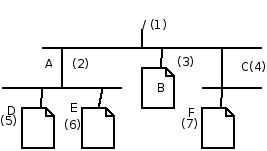
\includegraphics[width=0.6\linewidth]{memoire-images/fichiers-unix.png}

\begin{tabular}{|rcc|l|}
\hline
N° & type & CR & contenu des blocs \\
\hline
1 & d & 4 & ..$\rightarrow$1, .$\rightarrow$1, A$\rightarrow$2, B$\rightarrow$3, C$\rightarrow$4 \\
2 & d & 2 & ..$\rightarrow$1,.$\rightarrow$2, D$\rightarrow$ 5, E$\rightarrow$6 \\
3 & f & 1 & ``coucou'' \\
4 & d & 2 & ..$\*rightarrow$1, .$\rightarrow$4, F$\rightarrow$7 \\
% 5 & f & 1 & ``hello, world'' \\
& & \ldots & \\
\hline
\end{tabular}

Le compteur de références (CR) indique combien de fois un objet est
cité dans les répertoires. Quand il n'est plus cité, il est inaccessible
et donc on peut récupérer la place qu'il occupe.

\begin{exercice}
Sur ce schéma, étudiez l'effet successif des commandes
\begin{itemize}

\item \texttt{ ln /B /A/G}
\item \texttt{ rm /B }
\item \texttt{ rm /C/F}
\item \texttt{ mkdir /C/X }
\end{itemize}
\end{exercice}

\paragraph{Gestion des blocs libres}

Le système possède
\begin{itemize}
\item une liste des blocs libres
\item un tableau de marquage des blocs occupés
\end{itemize}



\paragraph{Vérification du système de fichiers}

L'utilitaire traditionnellement appelée \texttt{fsck} (\emph{File
  System ChecK}) sous UNIX effectue un parcours de l'arborescence, et
de la liste des blocs libres, pour en vérifier la cohérence.

\begin{enumerate}
\item vérification des i-noeuds, des blocs et des tailles
\item vérification de la structure des répertoires
\item vérification de la connectivité des répertoires
\item vérification des compteurs de référence
\item vérification de l'information du sommaire de groupe
\end{enumerate}

Certaines corrections sont effectuées automatiquement :
\begin{itemize}
\item
Dans le cas où des répertoires contiennent des références à des i-nodes
détruits, les références sont supprimées.
\item 
Dans le cas inverse où des i-nodes ``vivants'' ne sont plus référencés,
ils sont rattachés arbitrairement au répertoire ``\texttt{lost+found}''.
\end{itemize}

D'autres nécessitent l'intervention de l'administrateur, par exemple
quand des fichiers font usage de blocs qui sont marqués comme libres.
Il faut alors choisir entre supprimer le fichier, ou rattacher le bloc
au fichier.

\subsection{Autres caractéristiques des SGF}

Les systèmes de fichiers modernes ont d'autres fonctionnalités 
importantes.

\subsubsection{Journalisation}


\paragraph*{Journal} : 
\begin{itemize} 
\item garde une trace des opérations d'écriture non terminées
\item fournit un \emph{point de reprise} au cas où l'opération 
serait interrompue
(plantage, coupure de courant) pendant une écriture sur disque.
\end{itemize}

Avantages
\begin{itemize}
\item pas de pertes d'informations
\item reprise plus rapide (évite le \emph{fsck})
\end{itemize}



\subsubsection{Snapshots (instantané)}

Les ``instantanés'' sont des copies (virtuelles) de l'état du système
de fichiers à un moment donné.

\paragraph{Besoin} Ceci est utile 
en particulier pour les sauvegardes.  Quand on fait une
sauvegarde avec \texttt{tar} par exemple, ce programme établit la
liste des fichiers à sauvegarder avec leurs noms, leurs tailles etc,
puis construit une archive contenant cette liste et le contenu des
fichiers.

Or il se peut que les données à sauvegarder ``bougent'', parce que les
utilisateurs (ou des programmes) ajoutent, suppriment ou modifient les
fichiers entre la constitution de la liste et la construction de l'archive ;
ce qui peut conduire à une archive inexploitable.

\paragraph{Fonctionnement} 
Quand on demande un ``snapshot'', le SGF prend note de toutes les
modifications apportées au système de fichier ``actif'' à partir d'un
moment précis.  Le snapshot est constitué d'une table des sauvegardes
des blocs qui ont été modifiés sur le système de fichiers ``actif''.
Lorsqu'on demande le bloc numéro $n$ du snapshot, le SGF renvoie la
sauvegarde du bloc $n$ si il y en a eu une, et sinon le bloc $n$ du
système de fichiers.  La commande de sauvegarde peut donc, à travers
le ``cliché'', accéder aux données dans l'état où elles étaient à un
moment précis.

En quelque sorte, c'est une duplication partielle du système de
fichiers, au fur et à mesure des modifications ; le snapshop est
effectué instantanément (au moment de sa création, la table des
blocs modifiés est vide), et prend peu de place quand le système de
fichiers est peu actif.

\end{multicols}


